
%----------------------------------------------------------------%
%--------------------------GRUNDEINSTELLUNGEN--------------------%
%----------------------------------------------------------------%
\documentclass[oneside, ngerman, footinclude=off, captions=tableheading]{scrartcl}
%	'oneside'/'twoside': nicht zwischen linker und rechter Seite unterscheiden (alternativ twoside)
%	'twocolumn': wuerde 2 Spalten auf dem Blatt platzieren
%	'bibliography=totocnumbered': Normal nummeriertes Inhaltsverzeichnis (Kapitelnummer)
%	'listof=totocnumbered': Abbildungs- und Tabellenverzeichnis normal nummeriert (Kapitelnummer)
%	'ngerman' verwendet deutsch als Dokumentensprache (z.B. fuer Sirange)
%	'footinclude=off': Zaehlt Fusszeile zum Rand (vergroessert den Textbereich)
%	'captions=tableheading': Tabellenueberschriften explizit verwenden, erhoeht den Abstand zur Tabelle

\usepackage[ngerman]{babel}		%	Einstellen der Sprache
\usepackage[T1]{fontenc}		%	Wie wird Text ausgegeben, d.h. im PDF
\usepackage[utf8]{inputenc}		%	Welche Zeichen 'versteht' LaTeX bei der Eingabe?
\usepackage{lmodern}			%	Laedt Schriften, die geglaettet sind
\usepackage{blindtext}			%	Beispieltext, zum Testen geeignet

%----------------------------------------------------------------%
%--------------------------ABSTÄNDE------------------------------%
%----------------------------------------------------------------%
%\usepackage[onehalfspacing]{setspace}				%	Für Zeilenabstaende: 'singlespacing' (einfach), 'onehalfspacing' (1.5-fach), 'doublespacing' (2fach)
%\setlength{\parindent}{0cm}						%	Laengenangabe für die Einrueckung der ersten Zeile eines neuen Absatzes.
%\setlength{\parskip}{6pt plus 3pt minus 3pt}		%	Laengenangabe für den Abstand zwischen zwei Absaetzen.
%	Wenn diese beiden Befehle nicht kommentiert sind, wird ein Absatz nicht eingezogen sondern es gibt einen Abstand

% kleinere Abstände über und unter Gleichungen
\usepackage{setspace}\onehalfspacing
\AtBeginDocument{%
  \addtolength\abovedisplayskip{-0.2\baselineskip}
  \addtolength\belowdisplayskip{-0.2\baselineskip}
}

%----------------------------------------------------------------%
%--------------------------MATHE---------------------------------%
%----------------------------------------------------------------%
\usepackage[]{mathtools}							%	Erweiterung von AMSMath, laedt automatisch AMSMath - für viele Mathe-Werkzeuge, 'fleqn' als Option ist für Mathe linksbuendig
\usepackage{amsfonts}								%	Für eine Vielzahl an mathematischen Symbolen
\usepackage{nicefrac}

%----------------------------------------------------------------%
%--------------------------KOPF- UND FUSSZEILEN------------------%
%----------------------------------------------------------------%
\usepackage[automark,headsepline=.4pt]{scrlayer-scrpage}
\pagestyle{scrheadings}
\setkomafont{pageheadfoot}{\normalfont\bfseries}	%	Normale Schriftart und Fett für den Seitenkopf
\addtokomafont{pagenumber}{\normalfont\bfseries}	%	Normale Schriftart und Fett für die Seitenzahl
\clearpairofpagestyles								%	Löscht die Seitenkopf- und Seitenzahlen
\ohead{\thepage}									%	Rechter Seitenkopf mit Seitenzahl
\ihead{\headmark}									%	Linker Seitenkopf mit section
\ofoot[]{\empty}									%	Leere Fußzeile, ungerade Seiten
%	Definert man oben in der documentclass 'twoside', so wird zwischen geraden und ungeraden Seiten unterschieden (NUR DANN!)

%----------------------------------------------------------------%
%--------------------------BILDER--------------------------------%
%----------------------------------------------------------------%
\usepackage{graphicx}									%	Um Bilder einbinden zu koennen 
\usepackage[dvipsnames,svgnames,table]{xcolor}			%	Farben verwenden, Versch. Farbdefinitionen, Farben in Tabellen (-Reihen, -Spalten)
\usepackage{pdfpages}									%	pdfs importieren
\definecolor{Seeblau100}{RGB}{0,169,224}				%	Uni-Farben, z.B. fuer Tabellen
\definecolor{Seeblau65}{RGB}{89,199,254}
\definecolor{Seeblau35}{RGB}{165,224,254}
\definecolor{Seeblau20}{RGB}{203,237,254}
\definecolor{Seegrau60}{RGB}{102,102,102}
\definecolor{Seegrau40}{RGB}{153,153,153}
\definecolor{Seegrau20}{RGB}{204,204,204}
\definecolor{Seegrau10}{RGB}{230,230,230}

%----------------------------------------------------------------%
%--------------------------POSITIONIERUNG------------------------%
%----------------------------------------------------------------%
\usepackage{float}

%----------------------------------------------------------------%
%--------------------------LISTEN--------------------------------%
%----------------------------------------------------------------%
\usepackage{enumitem}							%	Um Listen / Aufzaehlungen leichter zu modifizieren
%\setlist{noitemsep}							%	Verringert den Abstand in Aufzaehlungen

%----------------------------------------------------------------%
%--------TABELLEN-/BILDUNTERSCHRIFTEN und NUMMERIERUNG-----------%
%----------------------------------------------------------------%
\addtokomafont{captionlabel}{\bfseries}			%	Abbildung X.Y wir fett geschrieben
\setcapindent{2em}								%	2. Zeile teilweise haengend und eingezogen. Wenn ganz haengend gewuenscht, auskommentieren


%----------------------------------------------------------------%
%--------------------------LITERATURVERZEICHNIS------------------%
%----------------------------------------------------------------%
\usepackage[german]{babelbib}					%	Bereitstellung des deutschen Layouts fuer die Bibliography
\bibliographystyle{babalpha}

%----------------------------------------------------------------%
%--------------------------SIUNITX-------------------------------%
%----------------------------------------------------------------%
\usepackage[]{siunitx}
\DeclareSIUnit\octave{oct}
\DeclareSIUnit\Hz{Hz}
\sisetup{locale = DE}							%	Automatische Einstellung der Ausgabe für bestimmte Regionen (UK, US, DE, FR, ZA)
\sisetup{separate-uncertainty = false
}

%----------------------------------------------------------------%
%--------------------------URLs / REFs---------------------------%
%----------------------------------------------------------------%
\usepackage[hidelinks]{hyperref}				%	Erweiterte Referenzierung ('hidelinks' verhindert Linien um Links)

%----------------------------------------------------------------%
%--------------------------EIGENE BEFEHLE------------------------%
%----------------------------------------------------------------%

\usepackage{todonotes}
\usepackage{wrapfig}
\setlength{\intextsep}{0pt}%
\usepackage{multicol}

\usepackage{listings}
\usepackage{xcolor}

\definecolor{codegreen}{rgb}{0,0.6,0}
\definecolor{codegray}{rgb}{0.5,0.5,0.5}
\definecolor{codepurple}{rgb}{0.58,0,0.82}
\definecolor{backcolour}{rgb}{0.95,0.95,0.92}

\lstdefinestyle{mystyle}{  
    commentstyle=\color{codegreen},
    keywordstyle=\color{magenta},
    numberstyle=\tiny\color{codegray},
    stringstyle=\color{codepurple},
    basicstyle=\ttfamily\footnotesize,
    breakatwhitespace=false,         
    breaklines=true,                 
    captionpos=t,                    
    keepspaces=true,                 
    numbers=left,                    
    numbersep=5pt,                  
    showspaces=false,                
    showstringspaces=false,
    showtabs=false,                  
    tabsize=2
}


\lstset{style=mystyle}


\begin{document}

\title{Computerphysik I: Blatt 03}
\author{Aurel Müller-Schönau und Leon Oleschko}
\maketitle


\section*{a) Magnetpendel - Erste Schritte}
Es soll ein Magnetpendel simuliert werden. Wir nehmen an, dass die Auslenkung klein ist, und beschränken uns auf die $x$-$y$-Ebene. Die auf die Stahlkugel wirkende magnetische Kraft soll von drei Magneten ausgehen und die form

\begin{align}
\vec{F}_m = \sum_{i=1}^N S_i \cdot \frac{\vec{r} - \vec{r}_i}{|r - r_i|^3}
\end{align}

Die individuelle Magnetstärke $S_i$ haben wir dabei selbst eingeführt, um das Programm für verschieden starke Magnete testen zu können. Sie wird aber im folgenden für alle Magnete $1$ betragen. $N$ ist die Anzahl der Magnete, $\vec{r}_i$ bezeichnet deren Position. Dabei haben wir uns im Programm bereits auf die $x$-$y$-Ebene beschränkt. Im Nenner kommt natürlich weiterhin auch die $z$-Komponente vor! Wie das praktisch aussieht, ist im Code im Anhang \ref{E_Pfad} zu sehen. Das Programm zeichnet den Pfad des Pendels für verschiedene Anfangspunkte, siehe dazu e). Im Programm werden die Koordinaten der Magneten in einem Array gespeichert, wobei die dritte Koordinate in wirklichkeit der Magnetstärke entspricht. Das Pendel befindet sich immer in der Höhe $h$ über der Magnetebene.\\
Zusätzlich soll eine Schwerkraft 

\begin{align}
\vec{F}_f = -k \vec{r}
\end{align}
\\
wirken, wobei wir $k=1$ wählen. Weiterhin soll eine Reibungskraft

\begin{align}
\vec{F}_r = -\gamma \dot{\vec{r}}
\end{align}
\\
das Pendel letztendlich zum Stillstand bringen.

\section*{b)}
Die Magnete wurden in einem regelmäßigen Dreieck im Abstand $1$ um den Ursprung angeordnet. Die Koordinaten betragen also $\left(\cos(\alpha), \sin(\alpha)\right)$ für $\alpha \in \{0, \frac{2\pi}{3}, \frac{4\pi}{3}\}$. Der Schwerpunkt liegt dann im Ursprung.

\section*{c)}
Die Simulation wurde im \textit{Leap-Frog-Verfahren} implementiert. Die Bewegungsgleichungen lauten dann

\begin{align}
&\vec{v}_{n+1} &= &\vec{v}_n &+ &H &\cdot &\vec{F}_{gesamt} / m \\\\
&\vec{r}_{n+1} &= &\vec{r}_n &+ &H &\cdot &\vec{v}_{n+1}
\end{align}
\\
Dabei wurde für die Beschleunigung $m=1$ gewählt. Im Programm \ref{E_Pfad} taucht $m$ deshalb gar nicht auf.

\section*{d)}
Bevor die eigentliche Simulation beginnen konnte, wurde das Programm zunächst mit verschiedenen Anfangswerten getestet. So musste etwa ein Bug gefixt werden, bei dem das Pendel immer am Nullpunkt zum stehen kam. Es stellte sich heraus, dass das Pendel zu hoch über der Magnetebene war, und die magnetische Kraft somit klein gegenüber der Schwerkraft war. Schließĺich konnte der Code auf zwei verschiedene Arten verwendet werden:

\section{e)}
Im Programm \ref{E_Path} befindet sich das Pendel in einer Höhe von $h=0.25$ Einheiten über der Magnetebene. Die Schwerkraftkonstante $K$ beträgt $1$, für die Dämpfung wurde $\gamma = 0.2$ gewählt. Dann wurden die Pfade dreier nahe beienanderliegender Startpunkte (keine Anfangsgeschwindigkeit) gezeichnet. Dies soll einen ersten Hinweis auf das chaotische Verhalten liefern. Die Anfangspunkte unterscheiden sich lediglich in der $x$-Koordinate um einen kleinen Wert $\pm \varepsilon$ mit $\varepsilon = 0.02$.\\
Das Ergebnis ist als Schaubild im Diagramm \label{fig:xy} dargestellt. Gezeichnet wurden die $x$-$y$-Diagramme der drei verschiedenen Startpunkte. Es ist zu erkennen, dass sich trotz anfänglich fast identischer Pfade die Pendelbewegung mit fortschreitender Zeit deutlich anders entwickelt.

\begin{figure}[t]
	\centering
	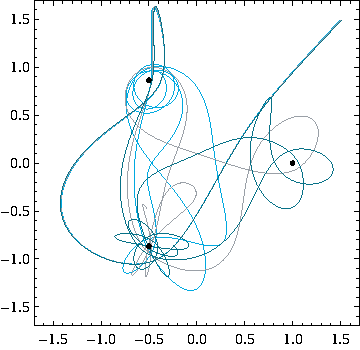
\includegraphics[width=290pt]{img/xy.pdf}
	\caption{$X$-$Y$-Diagramm eines losgelassenen Pendels für drei geringfügig verschiedene Startpunkte.}
	\label{fig:xy}
\end{figure}


\section*{f)}
Die Simulation im Programm \ref{F_Bild} ist identisch zu der im vorigen Teil, jedoch werden nun viele Punkte in der $x$-$y$-Ebene als Startpunkte gewählt. Für jeden Wert wird das Pendel ohne Anfangsgeschwindigkeit pendeln gelassen, bis es zum Stillstand gelangt, alternativ jedoch, falls $10000$ Simulationsschritte erreicht sind. Dann wird der Startpunkt des Pendels farbkodiert entsprechend dem Magneten, der dem Endpunkt am nächsten liegt. Die Positionen der Magnete sind dabei deutlich als große einfarbige Bereiche zu erkennen, ein hier losgelassenes Pendel pendelt erst gar nicht los.\\
Im Schaubild \ref{fig:Bild} ist das Ergebnis zu bestaunen.


\begin{figure}[t]
	\centering
	\includegraphics[width=290pt]{img/pfad2.pdf}
	\caption{Schaubild zur Illustration des chaotischen Verhaltens des Magnetpendels. Jeder Pixel im Bild stellt einen anderen Startpunkt dar. Die Farbe des jeweiligen Pixels entspricht dem Magneten, der dem Endpunkt am nächsten liegt. Die Magnete selbst sind mit Kreuzen markiert, und liegen in den drei großen einfarbigen Bereichen.}
	\label{fig:Bild}
\end{figure}

\clearpage
\section*{Appendix - Code}
\subsection*{c)}
\lstinputlisting[label={E_Pfad},caption={Programm zur Simulation des Magnetpendels für drei jeweils um $\varepsilon$ verschobene Startpunkte.},language=c]{path.c}

\clearpage
\subsection*{f)}
\lstinputlisting[label={F_Bild},caption={Simulation des Magnetpendels zum erstellen eines Schaubildes. Die Farbe im Bild kodiert den nächstgelegenen Magneten am Ende der Simulationszeit für den jeweiligen Startpunkt.},language=c]{magnetpendel.c}

\end{document}
